% Copyright Aidan Randle-Conde 2007-2014
% http://www.aidansean.com/phd_notes
% Anyone is free to download, redistribute, edit and use these notes and the source tex files with the following restrictions:
% This 
%  This message is included in the tex source files.
%  Aidan Randle-Conde is credited as the author.
%  Images are correctly credited to their respective authors, as outlined in the references.
%  No part of these notes may be used for commercial purposes.

\chapter{Experimental concepts}

\section{Experimental possibilities}

In reality there are rather few experiemental possibilities:
\begin{itemize}
  \item Scatter one particle off another and observe the reaction
  \item Generate a particle and observe subsequent decay processes
  \item Observe neutrino oscillations
  \item Measure a particle's properties eg charge, lifetime
\end{itemize}

\section{Cross sections}

The cross section, $\sigma$, is an imaginary area surrounding a ``target'' particle through which an incident particle must pass for a particular interaction to take place.

To calculate a cross section:
\begin{itemize}
  \item Assume $N_B$ particles per incident beam bunch
  \item Assume the beam illuminates an area $A$ of the target which is of length $l$ and density $\rho$
\end{itemize}

The number of target particles that are illuminated is:

\[
  N_T = \frac{lA\rho N_A}{m}
\]

where $m$ is the molecular mass of the target nuclei and $N_A$ is Avagadro's constant.

Each of the particles is imagined to have an area $\sigma$ surrounding it.  The probability that one beam particle interacts in the area $A$ is:

\begin{eqnarray*}
  P(\textrm{Interaction}) & = & \frac{l A\rho N_A}{m}\frac{\sigma}{A} \\
  & = & \frac{l \rho \sigma N_A}{m}
\end{eqnarray*}

The total number of interactions is then:

\[
  N_I = \frac{l \rho N_A N_B \sigma}{m}
\]

To avoid shadowing $N_I$ and $l$ are replaced by $\mathrm{d}N_I$ and $\mathrm{d}l$ respectively.  In order to calculate the number of interactions per second in a general collider it is necessary to make the expression symmetrical with respect to the beam and target:
\begin{itemize}
  \item Assume the particle densities in the beam and target are $\rho_B$ and $\rho_T$ respectively
  \item Assume the interactions are occuring in a volume $V$ with a cross-sectional area A
  \item Assume the beam travels with a relative speed $u$
\end{itemize}

The number of target particles in the volume $V$ is $\rho_T V$, so the probability of one beam particle interacting in the area $A$ is $\rho_T V \sigma / A$.  In $1\units{s}$ there are $uA\rho_B$ particles.

\[
  \Rightarrow \frac{\mathrm{d}n}{\mathrm{d}t} = u\sigma V \rho_B \rho_T
\]

In a collider there are $n$ bunches containing $N_B$ particles rotating at $u \sim c$.  A second beam rotates in the opposite direction.  The probability of an interaction is $\sigma N_B / A$ in one bunch of the second beam where $A$ is the cross-section interaction region.  In $1s$ $f$ bunches (where $f$ is the rotation frequency) pass through the bunch in the second beam:

\begin{eqnarray*}
  \Rightarrow \frac{\mathrm{d}N_I}{\mathrm{d}t} & = & \frac{f N_B N_B n \sigma}{A} \\
  & = & L \sigma
\end{eqnarray*}
where the luminosity, $L$, is given by:

\begin{eqnarray}
  L & = & \frac{n N^2_B f}{A} \nonumber \\
  L & = & \frac{1}{\sigma}\frac{\mathrm{d}N_I}{\mathrm{d}t} \label{eq:luminosity}
\end{eqnarray}

(\ref{eq:luminosity}) is the formal definition of the luminosty.  The unit of cross-section is the barn, where $1 bn = 10^{-28}\units{m}^2$ and the units of $L$ are $\units{bn}^{-1}\units{s}^{-1}$.  The luminosity can be quoted in inverse picobarns per second and the integrated luminosity can be quoted in inverse picobarns.

\subsection{Scattering pions and nucleons}

Pions and nucleaons interact strongly, with cross sections shown in figure \ref{fig:ch2_pionNucleonScattering}.  According to the old understanding of the strong interaction two protons may exchange a $\pi^0$ to form a $\Delta^{++}$ which subsequently decays to a proton and $\pi^0$, as shown in figure \ref{fig:ch2_PPToPPPi0}.

\begin{figure}[!htb]
  \begin{center}
    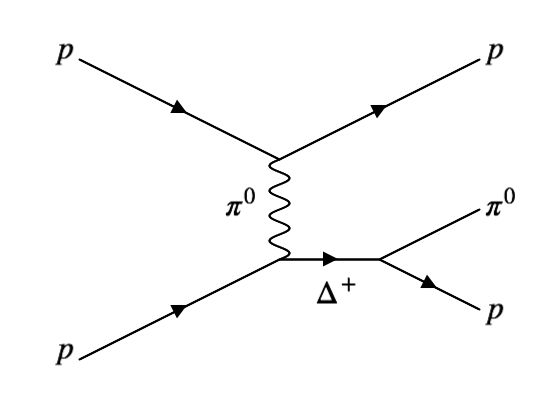
\includegraphics[width=0.8\textwidth]{images/web_feynman/image_8.png}
    \caption[Feynman diagram of proton-proton scattering]{Feynman diagram of proton-proton scattering, with the formation of the $\Delta^+$ resonance and emission of a $\pi^0$ meson.}
    \label{fig:ch2_PPToPPPi0}
  \end{center}
\end{figure}




\begin{figure}[!htb]
  \begin{center}
    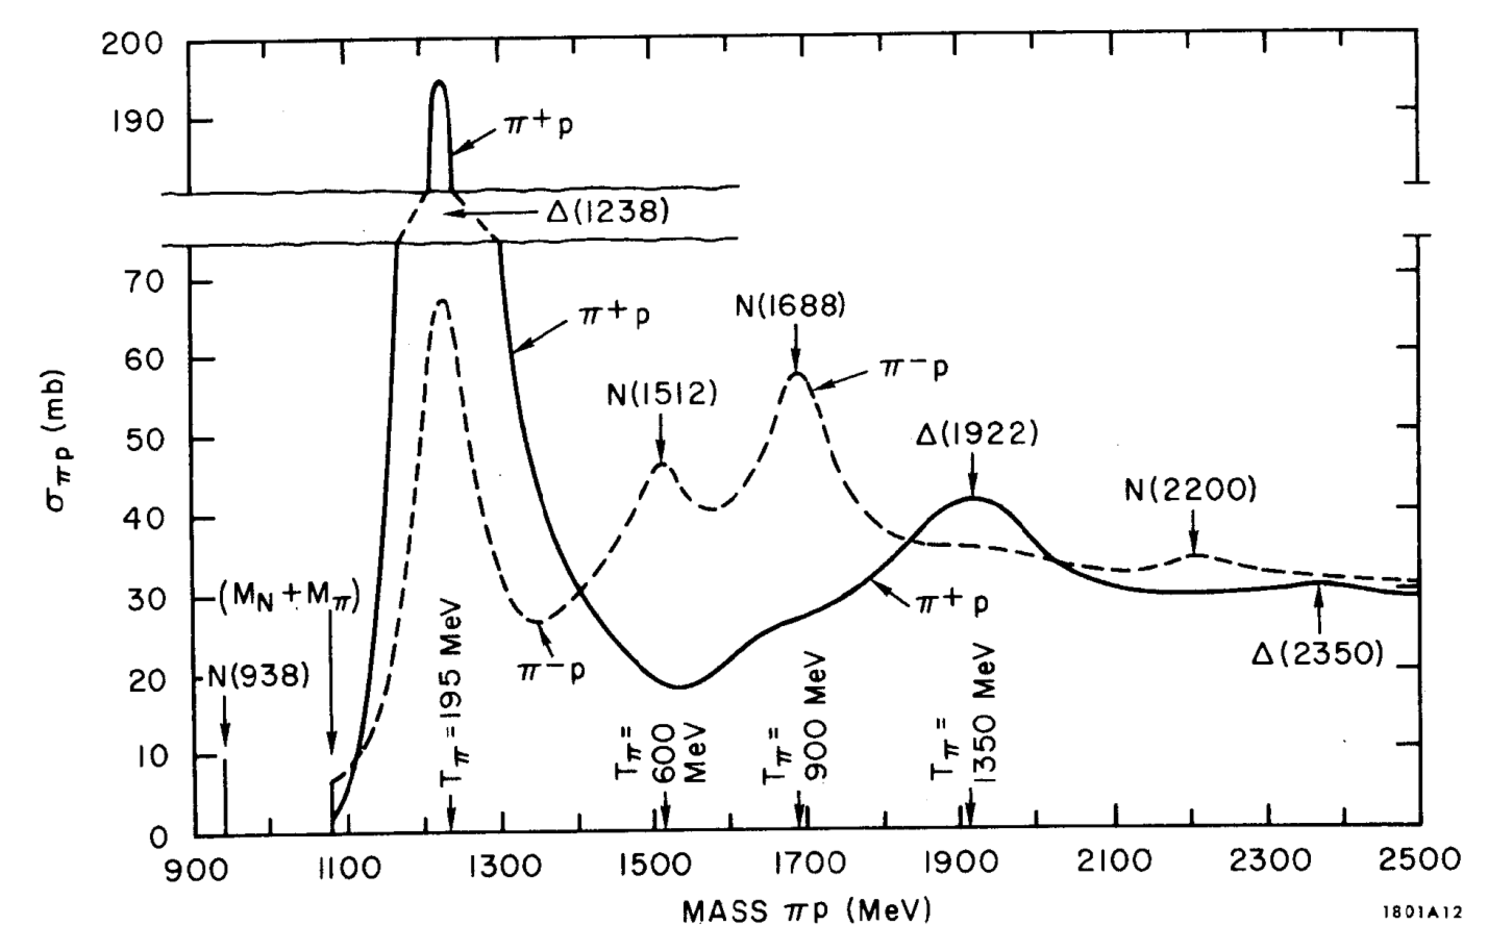
\includegraphics[width=\textwidth]{images/chapter_2/pionNucleonScattering.pdf}
    \caption[Pion-nucleon scattering cross section]{Pion-nucleon scattering cross section for positively and negatively charged pions incident on fixed targets. \cite{pionNucleonScattering}}
    \label{fig:ch2_pionNucleonScattering}
  \end{center}
\end{figure}

The cross sections for various interactions are:

\[
  \sigma_{pp} > \sigma_{np} \gg \sigma_{\gamma p} \gg \sigma_{\gamma \gamma}
\]

Detectors are based on such particle collisions and interactions and the radiation length is different for different materials eg high-energy electrons ($> \gev$) lose the same fraction of energy in $18 cm$ of water as in $2.8mm$ of lead.  In matter particles lose energy by ionisation, which is expressed as $\mathrm{d}E / \mathrm{d} x$, which is largely a function of the velocity of the particle, as shown in figure \ref{fig:ch2_energyLoss}.

\begin{figure}[!htb]
  \begin{center}
    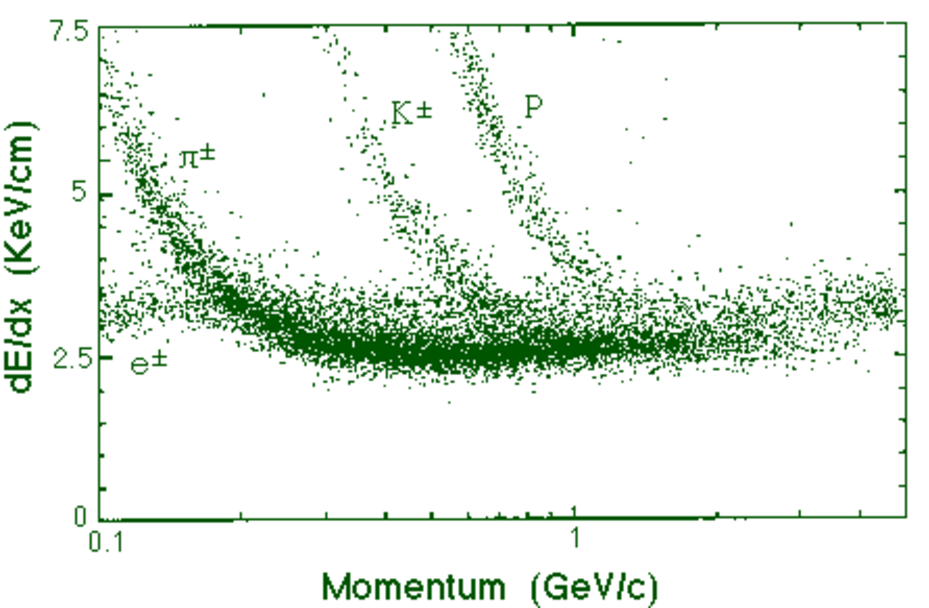
\includegraphics[width=0.5\textwidth]{images/chapter_2/Argus.pdf}
    \caption[Energy loss as a function of momentum]{Energy loss as a function of momentum, measured in the Argus drift chamber. \cite{energyLoss}}
    \label{fig:ch2_energyLoss}
  \end{center}
\end{figure}

\section{Natural units and conversion factors}

In quantum mechanics the expressions for energy and momentum can be expressed as:

\[
  \begin{array}{cccccl}
  E_{\nu} & = & hf & = & \hbar \omega    & \textrm{Planck's law} \\
  p_{\nu} & = & h/\lambda & = & \hbar k & \textrm{De Broglie's relation}
  \end{array}
\]

Travelling quantum waves are of the form:

\begin{eqnarray*}
  \psi & = & A \e^{i\left( kx - \omega t\right)} \\
  & = & A \e^{i/\hbar\left(px - Et\right)}
\end{eqnarray*}

And for light $c = f\lambda = \omega / k$.

It is conventient to set $\hbar = c = 1$.  Consider the units of $c\hbar$:

\begin{eqnarray*}
  [c\hbar] & = & [L] [T^{-1}] [E] [T] \\
  & = & [L] [E] \\
  c & = & 3 \times 10^8 \units{ms}^{-1} \\
  \hbar & = & 6 \times 10^{-25} \units{\gev s} \\
  c \hbar & = & 1.97 \times 10^{-16} \units{\gev m}
\end{eqnarray*}

Thus setting $c = \hbar = 1$ gives $1 = 1.97 \times 10^{-16} \gev\units{m}$.

Other useful conversion factors include:

\[
  \begin{array}{cccl}
  \frac{1}{\left( \gev \right)^2} & = & 3.89 \times 10^{-32}\units{m}^2 & = 0.389 \units{mb} \\
  \frac{1}{\gev} & = & 6.6 \times 10^{-5} \units{s} & 
  \end{array}
\]
